\documentclass{risepaper}
\卒論
%\修論
\usepackage{epsbox}
\usepackage{makeidx}
\usepackage[dvips]{graphicx}
\usepackage{fancybox}
  \title {Webベースグラフィカルプログラミングエディタを用いたFlexプログラミング環境の開発}        
   \author{尾崎 陽一}                                
\date{\today}
                                                          
\makeindex                                                
                                         
%\etitle{This is the English Title.}
% 2006/2/7改訂
% タイトルを複数行にしたいときは、下のetitleenv環境を使ってください。
\begin{etitleenv}
Development of a Flex Programming Environment 
using a Web-based Graphical Programming Editor
\end{etitleenv}

\begin{eabstract}
Flex is used for lexical analysis in the compiler exercise cource of this department.
The learners need to learn the grammar of Flex
in addition to concepts on lexical analysis.
However, Flex is a complex language that consists of 
the component to describe actions in the C language
and the regular expression part.
To learn two different concepts at the same time
is a heavy burden for beginners.
To resolve this problem, 
a Flex programming environment in which 
we do not have to be aware of the syntax is required.
There already exist such systems, one of which is  
A Graphical Programming Learning Support Environment using Adobe Flex.
However, since it is difficult to extend to languages
in which the control structure is significantly different compared with C,
it is not suitable as an environment for performing Flex programming.
This paper proposes a Flex programming environment in which 
beginners do not have to be aware of the syntax
using a Web-based graphical programming editor called Blockly.
It is easy to install because it is Web-based.
It is a scalable system and enables learners 
to shift to learning the syntax of Flex smoothly.
\end{eabstract}
 
\begin{jabstract}
本学科で開講されている「コンパイラ」の講義では、字句解析の演習にFlexが用いられる。
Flexを扱うためには、学習者はコンパイラの学習に加え、Flexの文法も学ぶ必要がある。
しかし、Flexは正規表現部とC言語の動作記述部とに分かれた複雑な言語である。
コンパイラの入門者にとって同時にこの二つを学ぶことは大きな負担となってしまう。
この問題を解決するには、文法を意識せずにFlexプログラミングが行える環境が必要となる。
既存のこのような環境として、Adobe Flexによるグラフィカルなプログラミング学習支援環境が
開発されている。
しかし、C言語と制御構造が大きく異なる言語に対しては拡張性に難があり、
Flexプログラミングを行う環境としては適していない。
本研究では、WebベースグラフィカルプログラミングエディタBlocklyを用いて文法を意識せずに行えるFlexプログラミング環境の開発を行った。
Webベースで導入が容易である。
また、Flexの文法学習にスムーズに移行でき、拡張性が高いシステムとなった。




\end{jabstract}


\begin{keyword}
プログラミング学習, Flex, Blockly, Webベース
\end{keyword}

\begin{document} 
\maketitle
%  \listoffigures % 図の目次
%  \listoftables  % 表の目次
                                                          
\chapter{はじめに}
\section{はじめに}

本学科で開講されている「コンパイラ」の講義では、字句解析の演習にFlexが用いられる。Flexは、正規表現とそれに対する動作記述から、C言語の字句解析プログラムを自動生成する字句解析器生成系
である。
Flexを扱うためには、学習者はコンパイラの学習に加え、Flexの文法も学ぶ必要がある。
しかし、Flexは以下のような点でコンパイラの入門者にとって難しい言語である。

\begin{itemize}
\item 正規表現部がどのような構造になっているのか分かりにくい
\item 正規表現部でエラーが発生した場合、実際にどの部分がエラーになっているのか分かりにくい
\item 特殊文字の扱いが難しい
\item 空白の有無によって意味が変わってしまうことがある
\end{itemize}

特に特殊文字の扱いについては、入門者にとって非常に難しい。
Flexではいくつかの文字は特殊文字として文法上特別な意味を持つ。
しかし、使用する個所によって特殊文字として扱われる場合や、そうでない場合が存在する。
この判別が、入門者にとって特に難しい部分である。
また、正規表現部と別にC言語で動作を記述する部分に分かれており複雑である。

学習者はコンパイラの学習と同時に複雑なFlexの文法を学ばなければならず、コンパイラの入門者にとって同時にこの二つを学ぶことは大きな負担となってしまう。

この問題を解決するには、文法を意識せずにFlexプログラミングが行える環境が必要となる。このような環境であれば、コンパイラの学習とFlexの文法の学習とを切り離すことができ、学習者はコンパイラの学習に集中して取り組むことができる。

既存の文法を意識せずにプログラミングを行える環境としては、本研究室で行われた先行研究として、
Adobe Flexによるグラフィカルなプログラミング学習支援環境の開発 \cite{Thesis01,Thesis02}が存在する。
ループや制御構造といった構文がグラフィカルパーツとして用意されており、
学習者はグラフィカルパーツを繋ぎあわせてプログラミングを行う。
このため文法を覚える必要が無く直感的にプログラミングを行うことができる。
また、グラフィカルパーツとC言語のソースコードの相互変換が可能である。
この機能により、グラフィカルパーツを利用するプログラミング学習から、
C言語といったプログラミング言語を用いた学習にスムーズに移行することができる。
さらに、JSON (JavaScript Object Notation) で記述を行うことにより、
柔軟なパーツ定義を可能としている。
しかし、C言語と制御構造が大きく異なる言語に対してはActionScriptで記述する必要がある。
FlexはC言語と制御構造が大きく異なるため、拡張性に難がある。

そこで本研究では、既存システムの問題点を解決するために、WebベースグラフィカルプログラミングエディタBlocklyを用いて文法を意識せずに行えるFlexプログラミング環境の開発を行う。

\section{先行研究}

\begin{itemize}
\item Scratch
\end{itemize}
Scratch \cite{Thesis03}はMITメディアラボが開発したプログラミング環境である。
図\ref{fig:Scratch}にScratchのイメージを示す。
ブロックを組み合わせて文法を意識せずにプログラミングを行うことができる。
Scratchは制御構造などのプログラムの基礎概念を学習するためのシステムであり、
本研究で求められている要件とは対象が異なる。
また、Scratchはスタンドアロンで動作するシステムでであり、インストール作業が必要である。
ただし、現在β版が公開されているScratch2.0では、Webベースアプリケーションになる予定である。
Webベースアプリケーションでは、インストール作業が不要である。
\newpage

\begin{figure}[h]
\begin{center}
\includegraphics[scale=0.3]{img/scratch.eps}
\caption{Scratch}%
\label{fig:Scratch}
\end{center}%
\end{figure}% 

\begin{itemize}
\item Adobe Flexによるグラフィカルなプログラミング学習支援環境
\end{itemize}

Adobe Flexによるグラフィカルなプログラミング学習支援環境 \cite{Thesis01,Thesis02}は、
プログラミング学習入門者を対象としたWebベースのプログラミング学習支援環境である。
図\ref{fig:sorada}にシステムのイメージを示す。
グラフィカルパーツによる文法を意識せずに行えるプログラミング方法と、
パーツとC言語のソースコードの相互変換によって、
プログラミングの基礎概念と、文法とを切り離して学習することができる。
JSONで記述を行うことにより、柔軟なパーツ定義が可能であるが、
制御構造が大きく異なる言語に対しては ActionScript で記述する必要があり、拡張性に難がある。

\newpage

\begin{figure}[h]
\begin{center}
\includegraphics[scale=0.5]{img/sorada.eps}
\caption{Adobe Flexによるグラフィカルなプログラミング学習支援環境}%
\label{fig:sorada}
\end{center}%
\end{figure}% 



\begin{itemize}
\item Waffle
\end{itemize}

Waffle \cite{Thesis04,Thesis05}はWebベースのFlex/Bisonプログラミング学習支援システムである。
図\ref{fig:Waffle}にWaffleのイメージを示す。
動的なハイライト表示を行うエディタによって、コーディング中における
Flex/Bisonの文法支援を行うことができる。
また、正規表現支援ツールにより、字句解析の理解の支援を行うことができる。
しかし、文法支援を受けるためにはまず学習者はエディタにソースコードを記述する必要がある。
そのため、ある程度Flex/Bisonの文法を理解し記述できる学習者でないと
システムを有効に扱うことができないという問題点がある。

\newpage

\begin{figure}[h]
\begin{center}
\includegraphics[scale=0.3]{img/Waffle.eps}
\caption{Waffle}%
\label{fig:Waffle}
\end{center}%
\end{figure}% 

\section{システムに求められる要件}

これらの先行研究の問題点を踏まえて、
本システムに求められる要件は以下のとおりである。
\begin{itemize}
\item 文法を意識せずにFlexプログラミング学習が行える
\item Flexの文法の学習へスムーズに移行できる
\item 導入が容易である
\item 拡張性が期待できるシステムである
\end{itemize}

コンパイラの学習とFlexの文法の学習とを切り離すために、
文法を意識せずにFlexプログラミングを行える必要がある。
本システムで字句解析の入門を学んだ後、Flexの文法の学習へとスムーズに移行できるのが望ましい。
また、入門者でも導入が容易に行えるように、Webベースシステムとして開発する。
そして、教員側から容易に拡張を行えるよう、拡張しやすいシステムでなければならない。

本論文では、第2章でBlocklyについて、第3章で実装したシステム、第4章でシステム評価、
第5章でまとめ、今度の課題について述べる。

\chapter{Blockly}
\section{Blockly}

\subsection{Blockly}
                                                          
Blocklyとは、Googleで開発されているグラフィカルなプログラミングエディタである。
図\ref{fig:Blockly}にBlocklyのイメージを示す。
ループや制御構造といった構文がブロックとして用意されており、このブロックを繋ぎあわせることでプログラミングを行うことができる。このため文法を覚える必要が無く直感的にプログラミングを行うことができる。

全てのコンポーネントはJavaScriptで記述されている。
ActionScriptは、記述したスクリプトをコンパイルしてSWFファイルに書き出さないと実行ができない。
しかし、JavaScriptは実行するためにコンパイルを行う必要は無い。
また、ドキュメントも豊富に用意されているため、
拡張性が高く、容易にカスタマイズを行うことができる。

また、BlocklyはWebベースのアプリケーションであるため、導入の作業が不要である。
学習者はWebブラウザがあればインストールや設定の必要なくシステムを利用できる。

さらに、Blocklyで作成したプログラムはJavaScriptなどの別の言語のコードに変換してリアルタイムに自動生成することができる。学習者は自分の作ったプログラムがどのようにソースコードで記述されるのかを確認しながらプログラミングを行うことができる。そのため、他の言語への移行性が高い。
現在はJavaScript, Dart, Pythonの三つの言語の出力をサポートしている。

\subsection{Waterbear}

1章で述べたシステムに求められる要件を満たす開発環境として、
Blocklyの他にWaterbear \cite{Thesis06}も考えられた。

WaterbearはScratchのようなブロックを使ったプログラミング言語を作成するためのツールキットである。
図\ref{fig:Waterbear}にWaterbearのイメージを示す。
Waterbearとはクマムシのことである。
クマムシはあらゆる環境の中でも生き残ることができる強靭な生き物であり、
クマムシのような堅牢なコードを作成できるようにとこの名前が付けられている。
Waterbear自体は言語そのものではなく、言語をブロックを使って視覚的に表すことができる。
HTML5、CSS3、JavaScriptを使って実装されており、
作成したプログラムはJavaScriptのコードとして常に確認することができる。

\begin{figure}[h]
\begin{center}
\includegraphics[scale=0.3]{img/Waterbear.eps}
\caption{Waterbear}%
\label{fig:Waterbear}
\end{center}%
\end{figure}% 

\subsection{開発環境}

Waterbearもまた、ブロックを用いてプログラミングを行うことができ、ソースコードの出力も可能なWebベースのシステムである。
Bloclyは、Canvas APIを使ってブロックを描画しているが、
Waterbearは HTMLとCSSを使ってブロックを描画している。
Waterbearは、ブロックの削除をBlocklyと比べて容易に行うことができ、
ユーザインタフェースの面で優れている。
しかし、Blocklyは、新たにブロックを作成する開発者のために、
ブロックを定義する関数が用意されている。
また、その関数を説明するドキュメントも豊富なため、Waterbearと比べてより容易にブロックの作成が可能である。本研究では、Flexという別の言語に対応させるために多くのブロックを作成する必要がある。
そのため、本研究では拡張性の面から開発環境としてBlocklyを選択した。

\begin{figure}[h]
\begin{center}
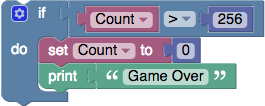
\includegraphics[scale=0.4]{img/blockly.eps}
\caption{Blockly}%
\label{fig:Blockly}
\end{center}%
\end{figure}% 

\section{システム構成}

Blocklyは、ワークスペース部、ブロックメニュー部、ソースコード部の3つのコンポーネントによって構成される。
ここでは、それぞれのコンポーネントについて説明する。

\subsection{ワークスペース部}

ワークスペース部は、ブロックを使ってプログラミングを行うスペースである。
図\ref{fig:workspase}にワークスペース部のイメージを示す。
ユーザは、ブロック部に存在するブロックをワークスペース部にドラッグアンドドロップによって移動させ、
それらのブロックを自由に組み合わせることによってプログラミングを行う。
ワークスペース部の右下にはゴミ箱のアイコンが存在する。
ワークスペースに設置したしたブロックをこのアイコンにドラッグすると、ブロックを削除することができる。

また、ワークスペース部に設置したブロックを右クリックすることで、以下のような動作が行える。

\begin{itemize}
\item ブロックの複製
\item コメントの追加
\item ブロックの接続表現の切り替え
\item ブロックの表現の簡略化
\item ブロックの透明化
\item ブロックの削除
\item ブロックの動作を説明するWebページを表示
\end{itemize}

\begin{figure}[h]
\begin{center}
\includegraphics[scale=0.4]{img/workspase.eps}
\caption{ワークスペース部}%
\label{fig:workspase}
\end{center}%
\end{figure}% 

\subsection{ブロックメニュー部}

ブロックメニュー部は、定義されたブロックが存在するスペースである。
図\ref{fig:menu}にブロックメニュー部のイメージを示す。
ブロックは制御構文を扱うブロック、数学関数を扱うブロックといったカテゴリーにそれぞれ格納され、
カテゴリー名をクリックすると格納メニューが現れる。
ユーザはその中から、自分の作成するプログラムに必要なブロックを選択して使用することができる。
ブロックがどのカテゴリーに属するかは、後述するブロックの定義方法で説明する。

\newpage

\begin{figure}[h]
\begin{center}
\includegraphics[scale=0.4]{img/menu.eps}
\caption{ブロックメニュー部}%
\label{fig:menu}
\end{center}%
\end{figure}% 

\subsection{ソースコード部}

ソースコード部は、作成したプログラムのソースコードを表示するスペースである。
図\ref{fig:source}にソースコード部のイメージを示す。
ワークスペース部にブロックを組み合わせて作成されたプログラムは、
リアルタイムにソースコードに変換され、このソースコード部でいつでも確認することができる。
この機能によって、Blocklyでプログラミングを学んだ学習者が他の言語の文法を学ぶ際、
文法の学習へスムーズな移行が可能となる。
現在は、JavaScript, Dart, Pythonの三つの言語のソースコードを出力することができる。
後述するソースコードの生成方法によって拡張を行うことで、
新たに定義したブロックや、新たな言語のソースコードを出力することも可能である。
また、プログラムの作成のために組み合わせたブロックの構造は、
このソースコード部にXML形式で出力される。
出力されたXMLコードをセーブ、ロードすることによって、組み合わせたブロックを保存したり、
他の学習者や教員が組み合わせたブロックを自分のワークスペース上に再現することができる。

\newpage

\begin{figure}[h]
\begin{center}
\includegraphics[scale=0.4]{img/source.eps}
\end{center}%
\caption{ソースコード部}%
\label{fig:source}
\end{figure}% 

\section{ファイル構成}

Blocklyは、以下のファイルで構成されている。

ファイル構成の説明

\begin{itemize}
\item demoフォルダ

Blocklyの起動を行うHTMLファイルとその設定ファイルで構成されている。
また、Blockly本体であるblockly\_compressed.jsファイルが存在する。

\end{itemize}

\begin{itemize}
\item generatorフォルダ

ソースコードの生成を行うプログラムで構成されている。

\end{itemize}

\begin{itemize}
\item languageフォルダ

各言語のブロックの定義を行うプログラムで構成されている。

\end{itemize}

\begin{itemize}
\item mediaフォルダ

ブロックの接続を行う際のサウンドエフェクトで構成されている。
\end{itemize}

\begin{itemize}
\item testsフォルダ

デバッグを行うプログラムで構成されている。

\end{itemize}

この他、以下のプログラムが存在する。

\shadowbox{
\begin{minipage}[t]{6cm}
\begin{verbatim}
block.js
block_svg.js
blockly.js
comment.js
connection.js
contextmenu.js
field.js
field_dropdown.js
field_label.js
field_textinput.js
flyout.js
generator.js
inject.js
mutator.js
names.js
procedures.js
scrollbar.js
toolbox.js
tooltip.js
trashcan.js
utils.js
variables.js
workspace.js
xml.js
\end{verbatim}
\end{minipage}
}

これらのプログラムは、build.pyファイルによってビルドされ、
demoフォルダのblockly\_compressed.jsに圧縮されている。

\section{ブロックの定義}

ここでは、Blocklyにおけるブロックの定義方法について述べる。

初めに、典型的な例としてテキストを記述するブロックの定義を以下に示す。

\shadowbox{
\begin{minipage}[t]{14cm}
\begin{verbatim}
Blockly.Language.text = {
  // Text value.
  category: Blockly.LANG_CATEGORY_TEXT,
  helpUrl: Blockly.LANG_TEXT_TEXT_HELPURL,
  init: function() {
    this.setColour(160);
    this.appendTitle('\u201C');
    this.appendTitle(new Blockly.FieldTextInput(''), 'TEXT');
    this.appendTitle('\u201D');
    this.setOutput(true, String);
    this.setTooltip(Blockly.LANG_TEXT_TEXT_TOOLTIP_1);
  }
};
\end{verbatim}
\end{minipage}
}

\begin{itemize}
\item カテゴリーの定義
\end{itemize}

作成したブロックがどのカテゴリーに属するのかを定義する。
カテゴリーの定義は以下のように行う。

\shadowbox{
\begin{minipage}[t]{8cm}
\begin{verbatim}
category: 'ここにカテゴリー名を記述する',
\end{verbatim}
\end{minipage}
}

同じカテゴリーに属するブロックは、ブロックメニュー部の同じメニューに格納される。
また、ここで新たなカテゴリー名を定義しても自動的にブロックメニュー部に新たなカテゴリーが追加される。

\begin{itemize}
\item ヘルプURLの定義
\end{itemize}

ブロックを右クリックした際行える動作として、ブロックの動作を説明するWebページを表示
する、というものがある。
ここでは表示するWebページを定義することができる。
ヘルプURLの定義は以下のように行う。

\shadowbox{
\begin{minipage}[t]{8cm}
\begin{verbatim}
helpUrl: 'ここにURLを記述する',
\end{verbatim}
\end{minipage}
}

Blocklyには新たなブロックを定義するためにいくつかの関数が用意されている。
以下にそれぞれの関数の機能と使用方法を示す。

\begin{itemize}
\item setColour

setColourは、ブロックの色を定義する関数である。
0から360までの範囲で数値を指定することで、ブロックの色を指定することができる。
setColourの使用例を以下に示す。

\shadowbox{
\begin{minipage}[t]{8cm}
\begin{verbatim}
this.setColour(160);
\end{verbatim}
\end{minipage}
}

\end{itemize}

\begin{itemize}
\item appendTitle

appendTitleは、ブロックにテキストを記述する関数である。
主に、各入力部が何を表すのかを記述するために使用する。
また、引数を変えることで、テキスト入力フィールド、ドロップダウンメニュー、
変数選択メニューなどを定義することも可能である。
appendTitleの使用例を以下に示す。

\shadowbox{
\begin{minipage}[t]{8cm}
\begin{verbatim}
this.appendTitle('hello');
\end{verbatim}
\end{minipage}
}

\end{itemize}

\begin{itemize}
\item appendInput


appendInputは、ブロックの入力を定義する関数である。
第二引数の値を変えることで入力を指定することができる。
また、appendTitleと同様にブロックにテキストを記述することができる。
appendInputの使用例を以下に示す。

\shadowbox{
\begin{minipage}[t]{12cm}
\begin{verbatim}
this.appendInput('', Blockly.INPUT_VALUE, 'ADD0', null);
\end{verbatim}
\end{minipage}
}

第一引数は記述するテキストの内容を指定する。
第二引数は入力方法を指定する。以下の3つから指定することができる。

\begin{itemize}
\item INPUT.VALUE

値を入力する接続部を定義する。
\end{itemize}
\begin{itemize}
\item NEXT.STATEMENT

接続されたブロックのステートを保持する接続部を定義する。
\end{itemize}
\begin{itemize}
\item DUMMY.INPUT

ダミーの入力を定義する。
実際には入力部は作成されない。
\end{itemize}

第三引数は接続部の名称を指定する。
ソースコードを生成する際、各入力部を区別するためにここで指定した名称を使用する。
第四引数は入力の型を指定する。
接続先のブロックの出力部の型とここで指定した入力部の型が一致したときのみ、
接続が行われるようになる。
型の指定が必要ない場合はnullを指定する。

\end{itemize}

\begin{itemize}
\item setOutput

setOutputは、ブロックの出力を定義する関数である。
この関数をブロックの定義に入れると、ブロックの左部に接続部が作成される。
この接続部は他のブロックの入力部に接続することができる。
setOutputの使用例を以下に示す。

\shadowbox{
\begin{minipage}[t]{8cm}
\begin{verbatim}
this.setOutput(true, String);
\end{verbatim}
\end{minipage}
}

第一引数はboolean型を指定する。falseを指定することもできるが、
その場合接続部が作成されないので、基本的にtrueを指定する。
第二引数は出力の型を指定する。
接続先のブロックの入力部の型とここで指定した出力部の型が一致したときのみ、
接続が行われるようになる。
型の指定が必要ない場合はnullを指定する。

\end{itemize}

\begin{itemize}
\item setPreviousStatement

setPreviousStatementは、文と文とを接続できるように
ブロックの上部に接続部を作成する関数である。
作成した接続部は、後述するsetNextStatementで作成した
接続部と接続することができる。
setPreviousStatementの使用例を以下に示す。

\shadowbox{
\begin{minipage}[t]{8cm}
\begin{verbatim}
this.setPreviousStatement(true);
\end{verbatim}
\end{minipage}
}

\end{itemize}

\begin{itemize}
\item setNextStatement

setNextStatementは、文と文とを接続できるように
ブロックの下部に接続部を作成する関数である。
作成した接続部は、前述したsetPreviousStatementで作成した
接続部と接続することができる。
setNextStatementの使用例を以下に示す。

\shadowbox{
\begin{minipage}[t]{8cm}
\begin{verbatim}
this.setNextStatement(true);
\end{verbatim}
\end{minipage}
}

\end{itemize}

\begin{itemize}
\item setTooltip

setTooltipは、ツールチップを定義する関数である。
文字列を記述すると、ユーザがブロックにカーソルを合わせたとき、
ここで記述した文字列が表示されるようになる。
setTooltipの使用例を以下に示す。

\shadowbox{
\begin{minipage}[t]{12cm}
\begin{verbatim}
this.setTooltip('A letter, word, or line of text.');
\end{verbatim}
\end{minipage}
}

\end{itemize}

\begin{itemize}
\item setInputsInline

setInputsInlineは、ブロックの接続表現を変える関数である。
Blocklyには、以下二つののブロックの接続表現が用意されている。
\begin{itemize}
\item External Inputs
\item Inline Inputs
\end{itemize}

図\ref{fig:Inline}にそれぞれの接続表現のイメージを示す。

\begin{figure}[h]
\begin{center}
\includegraphics[scale=0.8]{img/Inline.eps}
\caption{接続表現}%
\label{fig:Inline}
\end{center}%
\end{figure}% 

図\ref{fig:Inline}の左のブロックがExternal Inputs、右のブロックがInline Inputsである。
デフォルトではExternal Inputsに設定されているが、
変数を多く含むブロックの場合縦に大きくなってしまう。
このような場合、接続表現をInline Inputsにするとより簡潔にブロックを表現することができる。
setInputsInlineを使用すると、デフォルトの設定をInline Inputsに変えることができる。
また、接続表現の切り替えはワークスペース部で右クリックをすることで
ユーザ側からも可能である。
setInputsInlineの使用例を以下に示す。

\shadowbox{
\begin{minipage}[t]{8cm}
\begin{verbatim}
this.setInputsInline(true);
\end{verbatim}
\end{minipage}
}

\end{itemize}

\begin{itemize}
\item setMutator

setMutatorは、ミューテーターを定義するための関数である。
ミューテーターとは、Blocklyに用意されているブロックの形状を変更するための機能である。
図\ref{fig:mutator}にミューテーターを搭載しているブロックであるif文のブロックを示す。

\begin{figure}[h]
\begin{center}
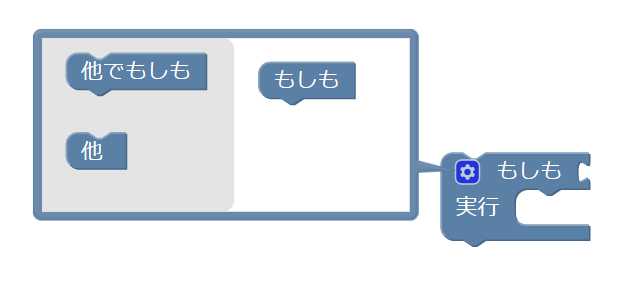
\includegraphics[scale=0.8]{img/mutator.eps}
\caption{ミューテーター}%
\label{fig:mutator}
\end{center}%
\end{figure}% 

図\ref{fig:mutator}の上部のブロックがif文のブロック本体である。
ブロック本体の左上の + が描かれている部分をクリックすると、
下部のエディットメニューが表示される。
ユーザはエディットメニュー内左部のelse if、elseを表すブロックを
エディットメニュー右部のif文のブロックに接続し上部のブロック本体に追加することができる。
例えば、elseブロックを接続すると、上部のブロック本体にifに加えてelseの接続部が追加される。
setMutatorの使用例を以下に示す。

\shadowbox{
\begin{minipage}[t]{14cm}
\begin{verbatim}
this.setMutator(new Blockly.Mutator
                    (['controls_if_elseif', 'controls_if_else']));
\end{verbatim}
\end{minipage}
}


\end{itemize}

\section{コード生成}

ここでは、定義したブロックからソースコードを生成する方法について述べる。

初めに、典型的な例としてWhile文を表すブロックのソースコード生成部の定義を以下に示す。

\shadowbox{
\begin{minipage}[t]{14cm}
\begin{verbatim}
Blockly.JavaScript.controls_whileUntil = function() {
  // Do while/until loop.
  var until = this.getTitleValue('MODE') == 'UNTIL';
  var argument0 = Blockly.JavaScript.valueToCode(this, 'BOOL',
      until ? Blockly.JavaScript.ORDER_LOGICAL_NOT :
      Blockly.JavaScript.ORDER_NONE) || 'false';
  var branch0 = Blockly.JavaScript.statementToCode(this, 'DO');
  if (until) {
    argument0 = '!' + argument0;
  }
  return 'while (' + argument0 + ') {\n' + branch0 + '}\n';
};
\end{verbatim}
\end{minipage}
}

ソースコードを生成するためには、まず、各入力部に入力されている引数を収集しなければならない。
Blocklyには引数を収集するためにいくつかの関数が用意されている。
以下にそれぞれの関数の機能と使用方法を示す。

\begin{itemize}
\item getTitleText

getTitleTextは、テキスト入力フィールドに入力されたテキストを収集する関数である。
appendTitleや、appendInputで定義されたテキスト入力フィールドに入力されたテキストを、
文字列としてコードを返す。
引数には、テキスト入力フィールドを作成した際に定義した名称を指定する。
getTitleTextの使用例を以下に示す。

\shadowbox{
\begin{minipage}[t]{8cm}
\begin{verbatim}
var code = this.getTitleText('TEXT');
\end{verbatim}
\end{minipage}
}

\end{itemize}

\begin{itemize}
\item getTitleValue

getTitleValueは、ドロップダウンメニューに指定した値を収集する関数である。
appendTitleや、appendInputで定義されたドロップダウンメニューから、
ユーザが選択したドロップダウン変数の名前を返す。
引数には、ドロップダウンメニューを作成した際に定義した名称を指定する。
getTitleValueの使用例を以下に示す。

\shadowbox{
\begin{minipage}[t]{12cm}
\begin{verbatim}
var until = this.getTitleValue('MODE') == 'UNTIL';
if (until) {
  argument0 = '!' + argument0;
}
\end{verbatim}
\end{minipage}
}

上の例では、MODEというドロップダウンメニューから
UNTILというドロップダウン変数がユーザによって選択された場合、untilという変数を作成する。
その後、untilが存在する場合に変数argument0に '!' を追加している。

\end{itemize}

\begin{itemize}
\item valueToCode

valueToCodeは、入力された値を収集する関数である。
指定した入力部にブロックが接続されていた場合、
接続されていたブロックの出力を文字列としてコードを返す。
valueToCodeの使用例を以下に示す。

\shadowbox{
\begin{minipage}[t]{14cm}
\begin{verbatim}
var argument0 = Blockly.JavaScript.valueToCode(this, 'FROM',
      Blockly.JavaScript.ORDER_ADDITION) || '0'
\end{verbatim}
\end{minipage}
}

上の例では、FROMという名称の入力部にブロックが接続されていると、
接続されていたブロックの出力を文字列として変数argument0に格納する。
ブロックが接続されていなかった場合、文字列 '0' を返す。
第三引数は、操作情報の順序を指定する。
各言語には演算子の優先順位が定義されている。
ここに、定義されている優先順位の中から操作に必要なものを指定する。

\end{itemize}

\begin{itemize}
\item statementToCode

statementToCodeは、入力されたステートメントを収集する関数である。
指定されたステートメントの入力部にブロックが接続されていた場合、
接続されていたブロックの出力を文字列としてコードを返す。
入力が接続されていない場合、空の文字列を返す。
statementToCodeの使用例を以下に示す。

\shadowbox{
\begin{minipage}[t]{14cm}
\begin{verbatim}
var branch0 = Blockly.JavaScript.statementToCode(this, 'DO');
\end{verbatim}
\end{minipage}
}

\end{itemize}


これらの関数によって収集した引数を使って、コードを生成することができる。
以下にJavaScriptのWhile文のソースコードの生成例を示す。

\shadowbox{
\begin{minipage}[t]{12cm}
\begin{verbatim}
return 'while (' + argument0 + ') {\n' + branch0 + '}\n';
\end{verbatim}
\end{minipage}
}

argument0とbranch0は収集した引数を格納した変数である。
argument0はvalueToCodeによって条件式に相当する値を格納している。
branch0はstatementToCodeによってwhile文の中の文に相当するステートを格納している。
これらの変数に、JavaScriptのWhile文のソースコードを表すように括弧や空白を追加していく。
必要な文字の追加は、通常の文字列と同じように行うことができる。
ソースコードが完成したら、return文として返す。


\chapter{システム実装}

本研究では、BlocklyでFlexプログラミングを行うために、以下のような実装を行った。

\section{ブロックの作成}

Flexは、Blocklyが本来サポートしている言語である
JavaScript, Dart, Pythonとは構造が大きく異なる言語である。
Flexプログラミングを行うためには、主に以下の動作が行える必要がある。

\begin{itemize}
\item 正規表現の記述
\item 動作の記述
\item 正規表現の定義
\item 関数の定義
\end{itemize}

そのため、Blockly上でFlexプログラミングを行うためには
これらの動作を行う新たなブロックを作成しなければならない。
また、各動作を繋げるためのブロックも必要である。

本節では、作成したブロックの機能と、その他に実装した機能について説明する。

\subsection{作成したブロック}

ここでは、作成したブロックの機能をカテゴリーごとに分けて説明する。

\begin{itemize}
\item 制御

制御カテゴリーは、Flexプログラミングを行う際の雛形となるブロックtempで構成されている。
制御カテゴリーのブロックのイメージを図\ref{fig:seigyo}に示す。

\begin{figure}[h]
\begin{center}
\includegraphics[scale=1.0]{img/seigyo.eps}
\end{center}%
\caption{制御カテゴリーのブロック}%
\label{fig:seigyo}
\end{figure}% 

tempブロックは、Flexプログラミングを行う際のベースとなる。
ユーザは定義、動作記述、関数のそれぞれのステート接続部に、
各カテゴリーのブロックを接続する形でプログラミングを行う。

\end{itemize}

\begin{itemize}
\item 正規表現

正規表現カテゴリーは、各正規表現を表す以下のブロックで構成されている。

\begin{itemize}
\item strブロック

strブロックは、文字列を記述するブロックである。
後述するitselfブロック、instrブロック、notstrブロック内に接続することができる。

\end{itemize}

\begin{itemize}
\item itselfブロック

itselfブロックは、strブロックを接続することで文字列そのものを表すブロックである。
Flexの文法では、文字列strそのものを示す以下の表記をこのブロックで表す。

\shadowbox{
\begin{minipage}[t]{4cm}
\begin{verbatim}
"str"
\end{verbatim}
\end{minipage}
}

\end{itemize}

\begin{itemize}
\item notstrブロック

notstrブロックは、文字列中の任意の文字を表すブロックである。
Flexの文法では、文字列str中の任意の文字を示す以下の表記をこのブロックで表す。

\shadowbox{
\begin{minipage}[t]{4cm}
\begin{verbatim}
[str]
\end{verbatim}
\end{minipage}
}

\end{itemize}

\begin{itemize}
\item rangeブロック

rangeブロックは、文字の範囲の任意の文字を表すブロックである。
Flexの文法では、文字c1から文字c2の範囲の任意の文字を示す以下の表記をこのブロックで表す。

\shadowbox{
\begin{minipage}[t]{4cm}
\begin{verbatim}
[c1-c2]
\end{verbatim}
\end{minipage}
}

\end{itemize}

\begin{itemize}
\item andorブロック

andorブロックは、正規表現の積和を表すブロックである。
Flexの文法では、正規表現r1と正規表現r2のandを示す
以下の表記をこのブロックで表す。

\shadowbox{
\begin{minipage}[t]{4cm}
\begin{verbatim}
r1r2
\end{verbatim}
\end{minipage}
}

また、正規表現r1と正規表現r2のorを示す以下の表記もこのブロックで表すことができる。

\shadowbox{
\begin{minipage}[t]{4cm}
\begin{verbatim}
r1|r2
\end{verbatim}
\end{minipage}
}

\end{itemize}

\begin{itemize}
\item loopブロック

loopブロックは、正規表現の繰り返しを表すブロックである。
Flexの文法では、正規表現rの0回以上の繰り返しを示す
以下の表記をこのブロックで表す。

\shadowbox{
\begin{minipage}[t]{4cm}
\begin{verbatim}
r*
\end{verbatim}
\end{minipage}
}

また、正規表現rの1回以上の繰り返しを示す以下の表記もこのブロックで表すことができる。

\shadowbox{
\begin{minipage}[t]{4cm}
\begin{verbatim}
r+
\end{verbatim}
\end{minipage}
}

\end{itemize}

\begin{itemize}
\item zeroneブロック

zeroneブロックは、正規表現の0回か1回の出現を表すブロックである。
Flexの文法では、正規表現rの0回か1回の出現を示す以下の表記をこのブロックで表す。

\shadowbox{
\begin{minipage}[t]{4cm}
\begin{verbatim}
r?
\end{verbatim}
\end{minipage}
}

\end{itemize}

正規表現カテゴリーのブロックのイメージを図\ref{fig:seiki}に示す。

\newpage

\begin{figure}[h]
\begin{center}
\includegraphics[scale=0.9]{img/seiki.eps}
\end{center}%
\caption{正規表現カテゴリーのブロック}%
\label{fig:seiki}
\end{figure}% 

ユーザはこれらのブロックを使って、正規表現部を記述することができる。
Flexには、正規表現部でエラーが発生した場合、実際にどの部分がエラーになっているのか
分かりにくいという問題があった。
しかし、本システムではブロックで正規表現を記述することができるので、
ユーザは構文エラーに悩まされることなくプログラミングを行うことができる。

また、ブロックの表現は、実際のFlexの文法のような記述形式としている。
日本語での記述形式の方が学習者の理解という点では優れている。
しかし、正規表現を記述するためにはこれらのブロックを多く使用しなければならない。
多くのブロックが接続された状態では、日本語での記述形式では横に長くなってしまい、
複雑になってしまう。
そのため、本研究ではより簡潔に表現が行えるFlexの文法のような記述形式としている。


\end{itemize}

\begin{itemize}
\item 動作

動作カテゴリーは、以下のブロックで構成されている。

\begin{itemize}
\item 正規表現部と動作記述部を接続するブロックconnect
\item 動作を記述するブロックbehavioral
\end{itemize}

動作カテゴリーのブロックのイメージを図\ref{fig:dousa}に示す。

\begin{figure}[h]
\begin{center}
\includegraphics[scale=1.0]{img/dousa.eps}
\end{center}%
\caption{動作カテゴリーのブロック}%
\label{fig:dousa}
\end{figure}% 

図\ref{fig:dousa}の上のブロックは、正規表現部と動作記述部を接続するブロックconnectである。
connectブロックの上の接続部には、正規表現カテゴリーのブロックを接続することができる。
下の接続部には、後述する動作を記述するブロックbehavioralを接続することができる。
また、connectブロックは制御カテゴリーのtempブロックの動作記述部に接続することができる。

図\ref{fig:dousa}の下のブロックは、動作を記述するブロックbehavioralである。
behavioralブロックにはテキスト入力フィールドが存在する。
ユーザはこのテキストフィールドにC言語で動作を記述することができる。

\end{itemize}

\begin{itemize}
\item 定義

定義カテゴリーは、正規表現の定義を行う以下のブロックで構成されている。

\begin{itemize}
\item 正規表現の定義を宣言するブロックfuncdif
\item 正義表現の定義を使用するブロックfunc
\end{itemize}

定義カテゴリーのブロックのイメージを図\ref{fig:teigi}に示す。

\newpage

\begin{figure}[h]
\begin{center}
\includegraphics[scale=1.0]{img/teigi.eps}
\end{center}%
\caption{定義カテゴリーのブロック}%
\label{fig:teigi}
\end{figure}% 

図\ref{fig:teigi}の上のブロックは、正規表現の定義を宣言するブロックfuncdifである。
funcdifブロックには、定義名を記述するためのテキスト入力フィールドが存在する。
また、定義する正規表現を接続するための接続部が存在する。
ユーザは定義したい正規表現を正規表現カテゴリーのブロックを使用して記述し、
この接続部に接続することで正規表現を定義することができる。
funcdifブロックは、制御カテゴリーのtempブロックの定義部に接続することができる。

図\ref{fig:teigi}の下のブロックは、正義表現の定義を使用するブロックfuncである。
funcdifブロックによって定義した正規表現は、funcブロックによって使用することができる。
funcブロックは、正規表現カテゴリーのブロックと自由に組み合わせることができる。

\end{itemize}

\begin{itemize}
\item 関数

関数カテゴリーは、yylex関数を呼び出すブロックyylexで構成されている。
関数カテゴリーのブロックのイメージを図\ref{fig:kansu}に示す。

\begin{figure}[h]
\begin{center}
\includegraphics[scale=1.0]{img/kansu.eps}
\end{center}%
\caption{関数カテゴリーのブロック}%
\label{fig:kansu}
\end{figure}% 

yylex関数とは、Flexが生成する字句解析関数のことである。
本来、Flexが生成したyylex関数は構文解析器で使用される。
本学科で開講されているコンパイラの講義では、Flexの演習が行われている。
この演習では、問題をより簡潔にするため、以下のようなmain関数を定義している。

\shadowbox{
\begin{minipage}[t]{8cm}
\begin{verbatim}
int main (void) {
  return yylex();
}
\end{verbatim}
\end{minipage}
}

このmain関数は、yylex関数を呼び出す関数である。
この関数をFlexのソースコードに定義することにより、
構文解析器を介さずFlex単体でyylex関数を呼び出すことができる。
本研究で作成したyylexブロックは、このmain関数を表すブロックである。
yylexブロックは、制御カテゴリーのtempブロックの関数部に接続することができる。


\end{itemize}


\subsection{オプション機能}

ユーザがFlexプログラミングを行いやすくなるよう、いくつかのオプション機能を実装した。
ここではオプション機能の詳細について説明する。

\begin{itemize}
\item ヘルプ機能

本研究では、正規表現を表すブロックの定義は、簡略化のために日本語での記述を省略した。
そのため、学習者がブロックの機能を理解しにくいという問題があった。
この問題を解決するため、setTooltip関数を使用してヘルプ機能を実装した。
ヘルプ機能のイメージを図\ref{fig:help}に示す。

\begin{figure}[h]
\begin{center}

\includegraphics[scale=1.0]{img/help.eps}
\end{center}%
\caption{ヘルプ機能}%
\label{fig:help}
\end{figure}% 

ブロックにカーソルを合わせることで、日本語の説明が表示される。
上の図のブロックは、正規表現rの0回か1回の出現を表すzeroneブロックである。
この機能によって、ユーザはブロックの使い方を容易に理解することができる。

\end{itemize}

\begin{itemize}
\item ブロックの接続補助

文法的に誤ったブロックの接続が行われないように型の定義を行った。
文字列を表す型Stringと、正規表現を表す型Regexp、動作を表す型Behaveを定義した。
String型を定義したのは以下のブロックである。

\shadowbox{
\begin{minipage}[t]{8cm}
\begin{verbatim}
strブロックの出力部
itselfブロックの入力部
instrブロックの入力部
notstrブロックの入力部
\end{verbatim}
\end{minipage}
}

Regexp型を定義したのは以下のブロックである

\shadowbox{
\begin{minipage}[t]{8cm}
\begin{verbatim}
itselfブロックの出力部
instrブロックの出力部
notstrブロックの出力部
rangeブロックの出力部
andorブロックの出力部
loopブロックの出力部
zeroneブロックの出力部
connectブロックの第一入力部
funcdifブロックの入力部
funcブロックの出力部
\end{verbatim}
\end{minipage}
}

Behave型を定義したのは以下のブロックである。

\shadowbox{
\begin{minipage}[t]{8cm}
\begin{verbatim}
connectブロックの第二入力部
behavioralブロックの出力部
\end{verbatim}
\end{minipage}
}

入力部と出力部の型が違う場合、接続が行われない。
例えば、String型であるitselfブロックの入力部には
Regexp型であるinstrブロックの出力部を接続することはできない。
この機能により、ユーザは常に文法的に正しいブロックの接続を行うことができる。

\end{itemize}

\section{Flexコードの自動生成}

\subsection{Flexコードの自動生成}

第2章で述べたとおり、Blocklyにはユーザが繋ぎあわせたブロックからリアルタイムに
ソースコードを自動生成する機能がある。
今回の研究では、この機能に新たに作成したブロックから
Flexコードを自動生成できるように拡張した。
実装には、2.4節で述べた関数を使用した。

図\ref{fig:blocksample}は、入力ファイル中の「aloha」「Aloha」という文字列を「namaste」に書き換える
Flexプログラムを本システムで作成したイメージである。

\newpage

\begin{figure}[h]
\begin{center}
\includegraphics[scale=0.5]{img/blocksample.eps}
\end{center}%
\caption{プログラム例}%
\label{fig:blocksample}
\end{figure}% 

本システムは、図\ref{fig:blocksample}のブロックから以下のソースコードを生成する。

\begin{figure}[h]
\begin{center}
\includegraphics[scale=0.5]{img/sourcesample.eps}
\end{center}%
\caption{ソースコード例}%
\label{fig:sourcesample}
\end{figure}% 

本システムはFlexプログラミングの入門者を対象としているため、複雑な字句解析プログラムを作ることはできない。より複雑な字句解析プログラムの作成には、Flexの文法の学習が必要である。
本システムではブロックでのプログラミングがリアルタイムにソースコードに反映されるため、
ユーザがFlexの文法学習に移行しやすい。

\subsection{インデントを行う問題の改善}

Blocklyでは、setPreviousStatement関数、setNextStatement関数によってステートを
接続する接続部を作ることができる。
この接続部を使って文と文とを接続すると、自動的にインデントが行われ、空白が挿入される。
Blocklyが本来サポートしているJavaScript, Dart, Pythonといった言語では、
このインデント機能は有効な機能である。
しかし、Flexにおいては空白が挿入されることによって意味が変わってしまうことがある。
例えば、正規表現の定義を記述する場合、
定義名は行の先頭から始まる。
そのため、行の先頭にインデントが行われてしまうと、定義名が変わってしまい、問題がある。

Blocklyでインデントを行っている部分は、generator.jsのGenerator.get関数である。
Generator.get関数では、以下の部分でインデントを行っている。

\shadowbox{
\begin{minipage}[t]{12cm}
\begin{verbatim}
if (code) {
    code = Blockly.Generator.prefixLines(code, '  ');
}
\end{verbatim}
\end{minipage}
}

if文の条件のcodeは、ステートが接続されているか判定している部分である。
prefixLinesは、行頭に文字列を挿入する関数である。
この部分では、ステートが接続されていた場合、行頭に空白を挿入してインデントを行っている。
本研究ではこの部分をコメントアウトし、インデントが行われないように改善した。


\chapter{評価}
\section{評価}

香川研究室の学部生3名を対象に、本システムの評価を行った。
本章では、システム評価について述べる。

\subsection{項目}

実際にシステムを使用してもらい、その後以下の項目に自由に回答する形式で行った。
\begin{itemize}
\item 操作方法は直感的に分かりましたか
\item 従来の方法と比べてどうでしたか
\item 分かりにくいブロックの表現はありませんでしたか
\item その他欲しい機能など
\end{itemize}

\subsection{結果}

評価の結果、良かった点として次のような意見が挙がった。
\begin{itemize}
\item 直感的に操作方法が分かった
\item エディタでプログラミングを行うのとくらべて分かりやすかった
\item ブロックの接続の可否によって文法の間違いがあらかじめ分かるのが良い
\end{itemize}

一番上は、システム自体の操作方法についての意見である。
システムを見ただけで操作の方法が直感的に分かるかということは、
学習支援を行う上で重要である。
直感的に操作方法が分かったという意見が得られたことは高評価であるといえる。

次は、従来の方法と比べてどうだったかという意見である。
従来のエディタでプログラミングを行うのと比べて分かりやすかったという意見が得られた。
ブロックによる直感的なプログラミングや、日本語の説明の表示によって
学習者の支援が行えたといえる。

最後は、ブロックの接続補助についての意見である。
本システムでは、型の定義によって、文法的に間違ったブロックの接続が行われないようにした。
この機能によって、学習者の間違いを減らすことができたといえる。

また、悪かった点として次のような意見が挙がった。
\begin{itemize}
\item 正規表現のandを示すブロックが何を意味しているのか分かりにくい
\item 動作を表すブロックに何を記述すべきか分からなかった
\item 接続できないブロックを区別する方法が欲しい
\end{itemize}

上の二点は、ブロックの表現方法についての意見である。
ブロックが長くならないように表現を簡潔にしたが、学習者にとっては分かりにくく感じたようである。
これらのブロックの表現方法については、改善が必要である。

次は、ブロックの接続補助についての意見である。
文法的に間違ったブロックの接続が行われないことで、学習者の間違いを減らすことができたが、
どのブロックが接続可能なのか表現する方法が学習者には必要であることが分かった。
接続部の形を変えるなどの方法で、視覚的に理解できる方法の検討が必要である。


\chapter{おわりに}
\section{まとめ}

コンパイラ学習者の支援のために、
WebベースグラフィカルプログラミングエディタBlocklyを用いてFlexプログラミング環境を開発した。
Webベースで導入が容易であり、学習者は文法を意識せずにFlexプログラミングを行うことができる。
また、リアルタイムにFlexのソースコードが確認でき、学習者はFlexの文法学習にスムーズに移行できる。
全てのコンポーネントはJavaScriptで記述されており、容易にカスタマイズを行うことができる。
これらの特徴は、1章で述べたシステムに求められる要件を満たしているといえる。

本研究で実装したシステムのイメージを図\ref{fig:blocklyimage}に示す。

\begin{figure}[h]
\begin{center}
\includegraphics[scale=0.4]{img/blocklyimage.eps}
\end{center}%
\caption{実装したシステム}%
\label{fig:blocklyimage}
\end{figure}% 


\section{今後の課題}

以下に本システムの今後の課題を述べる。

\begin{itemize}
\item プログラムの実行

本研究で開発を行ったシステムは、Flexのソースコードの生成を行うことができる。
しかし、現段階では生成したソースコードの実行を行うことができない。
Flexプログラミング入門者の支援をより行うためには、システム内でプログラムを実行可能にして
動作を確認できることが望ましい。
そのためには、サーバーサイドを実装することが必要である。
サーバーサイドの実装には、WappenLite \cite{Thesis07}を利用する予定である。
WappenLiteは、本研究室で開発されたWebベースの
プログラミング環境構築のためのフレームワークである。
WappenLiteと連携を行うことでシステム内でブログラムが実行可能になる。

\end{itemize}

\begin{itemize}
\item Bisonへの対応

実際のコンパイラの演習では、Flexと同時に構文解析器生成系であるBisonも用いられている。
演習内ではBisonとFlexを併用しプログラムを作成する場面もある。
また、BisonもBNFと動作記述とに分かれた文法的に難しい言語である。
そのため、よりコンパイラ学習者の支援を行うには、
Bisonについても文法を意識せずにプログラミングを行える環境が必要であると考えられる。

\end{itemize}

\begin{itemize}
\item ブロックの表現方法の改善

評価の結果、学習者が分かりにくいと感じるブロックの表現方法がいくつか挙がった。
学習者がブロックの機能をすぐに理解できるように、
ブロックの表現方法について検討する必要がある。
ただし、複数のブロックを組み合わせても煩雑にならないよう、できるだけ簡略化しなければならない。

\end{itemize}

\begin{itemize}
\item ブロックの機能の拡張

いくつかのブロックについて、以下のような拡張が必要である。

\begin{itemize}
\item 特殊文字に関する支援

現在のシステムでは、特殊文字に関する支援が行われていない。
Flexでは、以下の文字は文法上特別な意味を持つ特殊な文字である。

\shadowbox{
\begin{minipage}[t]{8cm}
\begin{verbatim}
\ " . [ ] * + ? { } | ( ) - < > ^ % / $
\end{verbatim}
\end{minipage}
}

Flexのコードの多くの箇所では、これらの文字は特殊文字として扱われる。
しかし、例外も存在する。
例えば、文字列str中の任意の文字を表す正規表現は、Flexでは以下のように表記される。

\shadowbox{
\begin{minipage}[t]{4cm}
\begin{verbatim}
[str]
\end{verbatim}
\end{minipage}
}

この正規表現の括弧内は、「]」, 「\verb|^|」,「-」,「\verb|\|」を除く特殊文字は
特別な意味を持たない。
入門者にとって、この特殊文字の例外は難解である。
特殊文字として扱う個所はソースコードを生成する際に自動で特殊文字として扱う、
といった機能を実装して支援を行う必要がある。

\end{itemize}

\begin{itemize}
\item 関数の定義

関数カテゴリーにyylex関数を呼び出す関数が用意されているが、
ユーザ側から新たな関数を定義することができない。
より多様なFlexプログラミングを行うためには、システム内で関数を定義できなくてはならない。
そのため、関数を定義するためのブロックを作成し、
ユーザの自由な関数定義を可能とする必要がある。

\end{itemize}

\end{itemize}

\begin{itemize}
\item 入力部の自動追加

本研究では、正規表現カテゴリーに、
文字の範囲の任意の文字を表すブロックrangeを定義した。
本来のFlexの文法では、以下のように括弧内には複数の文字の範囲を記述することが可能である。

\shadowbox{
\begin{minipage}[t]{4cm}
\begin{verbatim}
[a-zA-Z0-9]
\end{verbatim}
\end{minipage}
}

しかし、現在のrangeブロックでは一つの範囲しか記述することができない。

また、正規表現の積和を表すブロックandorを定義した。
現在のシステムでは、ユーザが新たに関係を追加しようとするたびに
andorブロックを生成し、接続しなければならない。
この問題の解決には、自動的に追加の入力部を生成する機能が必要である。
ミューテーター機能によって形状を変更し、入力部を複数に追加することは可能である。
しかし、この場合エディットメニューを開く手間が生じてしまう。

\end{itemize}

\begin{itemize}
\item ブロックの延長の改善

本システムでは、ブロックを組み合わせてFlexプログラミングを行うことができる。
ブロックは簡潔な表現を行ってはいるものの、より多くのブロックが接続されると横に長くなってしまう。
ブロックが画面を超える長さになってしまうと、スクロールさせねばならず手間が生じる。
ある程度の長さになると自動的に改行する機能が必要である。

\end{itemize}

\begin{itemize}
\item 接続部の形の変更

評価の結果、接続できないブロックの場合、接続できるブロックと区別する方法が欲しいという
意見が挙がった。
学習者がより直感的にプログラムを行うためには、接続部の形をいくつか用意し、
この二つのブロックの区別をはっきりと示す必要がある。
また、分かりやすい接続部の形について検討しなければならない。

\end{itemize}

\acknowledgment  % 謝辞

本研究においてご指導を賜りました香川考司教員に心から感謝の意を表します。

また,評価にご協力いただいた香川研究室の鳥原悠平君、藤沢尚樹君、森田昌樹君に深く感謝します。

\begin{thebibliography}{99} % 参考文献
                                  
 \bibitem{Thesis01} % 論文
 空田 卓也・香川 考司, 
 ``Adobe Flexによるグラフィカルなプログラミング学習支援環境,'' 
 教育システム情報学会研究報告 25(3), 香川大学 幸町キャンパス, pp. 3-6, 2010.

 \bibitem{Thesis02} % 論文
 空田 卓也, 
 ``拡張可能なグラフィカルプログラミング学習支援環境の開発,'' 
 香川大学大学院工学研究科2011年度修士論文, 2012.

 \bibitem{Thesis03} % 論文
 John Maloney, Leo Burd, Yasmin Kafai, Natalie Rusk, Brian Silverman and Mitchel Resnick,
 ``Scratch: A Sneak Preview,''
 Second International Conference on Creating, Connecting, and Collaborating through 
 Computing. Kyoto, Japan, pp. 104-109, 2004.

 \bibitem{Thesis04} % 論文
 中山 和也・香川 考司,
 ``AMFを利用したプログラミング学習支援システム,'' 
 教育システム情報学会研究報告 25(3), 香川大学 幸町キャンパス, pp. 7-12, 2010.

 \bibitem{Thesis05} % 論文
 中山 和也,
 ``WebベースのFlex/Bisonプログラミング学習支援システムWaffleの開発,'' 
 香川大学大学院工学研究科2011年度修士論文, 2012.

 \bibitem{Thesis06} % 論文
 Dethe Elza, ``Waterbear: Welcome,''
 http://waterbearlang.com/,2013年2月15日閲覧

 \bibitem{Thesis07}
 Koji Kagawa, ``WappenLite: a Web Application Framework for Lightweight Programming Environments,''
  9th International Conference on Information Technology Based Higher Education and Training (ITHET 2010),
  April 2010, Cappadocia, Turkey, pp.21-26.

\end{thebibliography}

\appendix         % 付録
\chapter{プログラムの一部ソース}

\section{ブロック部 testblock.js}

\small
\begin{verbatim}
if (!Blockly.Language) Blockly.Language = {};

Blockly.Language.temp = {
  //テンプレート.
  category: '制御',
  init: function() {
    this.setColour(180);
    this.appendTitle('最初にこのブロックを設置してください', 'NAME');
    this.appendInput('定義', Blockly.NEXT_STATEMENT, 'DO0');
    this.appendInput('動作記述', Blockly.NEXT_STATEMENT, 'DO1');
    this.appendInput('関数', Blockly.NEXT_STATEMENT, 'DO2');
  }
}

Blockly.Language.test_str = {
  // 文字列
  category: '正規表現',
  //helpUrl: Blockly.LANG_TEXT_TEXT_HELPURL,
  init: function() {
    this.setColour(180);
    this.appendTitle('文字列');
    this.appendTitle(new Blockly.FieldTextInput(''), 'TEXT');
    this.setOutput(true, String);
    this.setTooltip('文字列です');
  }
};

Blockly.Language.test_str_itself = {
  //文字列そのもの
  category: '正規表現',
  //helpUrl: Blockly.LANG_MATH_NUMBER_HELPURL,
  init: function() {
    this.setColour(300);
    this.setOutput(true, "Regexp");
    this.appendInput('"', Blockly.INPUT_VALUE, 'TEXT', String);
    this.appendInput('"', Blockly.DUMMY_INPUT, '');
    this.setInputsInline(true);
    this.setTooltip('中に文字列を入れると、文字列そのものを表します');
  }
};

Blockly.Language.test_instr = {
  //文字列中の任意の文字
  category: '正規表現',
  //helpUrl: Blockly.LANG_MATH_NUMBER_HELPURL,
  init: function() {
    this.setColour(300);
    this.setOutput(true, "Regexp");
    this.appendInput('[', Blockly.INPUT_VALUE, 'TEXT', String);
    this.appendInput(']', Blockly.DUMMY_INPUT, '');
    this.setInputsInline(true);
    this.setTooltip('中に文字列を入れると、その文字列中の任意の文字を表します');
  }
};

Blockly.Language.test_notstr = {
  //文字列に含まれない任意の文字
  category: '正規表現',
  //helpUrl: Blockly.LANG_MATH_NUMBER_HELPURL,
  init: function() {
    this.setColour(300);
    this.setOutput(true, "Regexp");
    this.appendInput('[^', Blockly.INPUT_VALUE, 'TEXT', String);
    this.appendInput(']', Blockly.DUMMY_INPUT, '');
    this.setInputsInline(true);
    this.setTooltip('中に文字列を入れると、その文字列に含まれない任意の文字を表します');
  }
};

Blockly.Language.test_range = {
  //文字の範囲の任意の文字
  category: '正規表現',
  //helpUrl: Blockly.LANG_MATH_NUMBER_HELPURL,
  init: function() {
    this.setColour(300);
    this.setOutput(true, "Regexp");
    //中に別に文字ブロックを入れる形式
    /*this.appendInput('[', Blockly.INPUT_VALUE, 'FROM', String);
    this.appendInput('-', Blockly.INPUT_VALUE, 'TO', String);
    this.appendInput(']', Blockly.DUMMY_INPUT, '');*/
    this.appendTitle('[');
    this.appendTitle(new Blockly.FieldTextInput(''), 'FROM');
    this.appendTitle('-');
    this.appendTitle(new Blockly.FieldTextInput(''), 'TO');
    this.appendTitle(']');
    this.setInputsInline(true);
    this.setTooltip('左の文字から右の文字の範囲の任意の文字を表します');
  }
};

Blockly.Language.test_and_or = {
  //正規表現 r1 の後に、もしくはまたは正規表現 r2
  category: '正規表現',
  //helpUrl: Blockly.LANG_MATH_NUMBER_HELPURL,
  init: function() {
    this.setColour(300);
    this.setOutput(true, "Regexp");
    this.appendInput('', Blockly.INPUT_VALUE, 'A', "Regexp");
    var dropdown = new Blockly.FieldDropdown([['', 'AND'], ['|', 'OR']])
    this.appendInput([dropdown, 'OP'], Blockly.INPUT_VALUE, 'B', "Regexp");
    this.setInputsInline(true);
    this.setTooltip('正規表現の後に(または)正規表現を繋げます');
  }
};

Blockly.Language.test_loop = {
  //正規表現rの繰り返し
  category: '正規表現',
  //helpUrl: Blockly.LANG_MATH_NUMBER_HELPURL,
  init: function() {
    this.setColour(300);
    this.setOutput(true, "Regexp");
    this.appendInput('', Blockly.INPUT_VALUE, 'TEXT', "Regexp");
    var dropdown = new Blockly.FieldDropdown([['*', '*'], ['+', '+']])
    this.appendInput([dropdown, 'OP'], Blockly.DUMMY_INPUT, '');
    this.setInputsInline(true);
    this.setTooltip('正規表現0回または1回以上の繰り返しを表します');
  }
};

Blockly.Language.test_zerone = {
  //正規表現rの0回か1回の出現
  category: '正規表現',
  //helpUrl: Blockly.LANG_MATH_NUMBER_HELPURL,
  init: function() {
    this.setColour(300);
    this.setOutput(true, "Regexp");
    this.appendInput('', Blockly.INPUT_VALUE, 'TEXT', "Regexp");
    this.appendInput('?', Blockly.DUMMY_INPUT, '');
    this.setInputsInline(true);
    this.setTooltip('正規表現の0回または1回の出現を表します');
  }
};

Blockly.Language.connect = {
  //動作記述
  category: '動作',
  init: function() {
    this.setColour(250);
    this.appendInput('正規表現', Blockly.INPUT_VALUE, 'REGEXP', "Regexp");
    this.appendInput('のとき', Blockly.INPUT_VALUE, 'TEXT', "Behave");
    this.setPreviousStatement(true);
    this.setNextStatement(true);
  }
}

Blockly.Language.behavioral = {
  //動作
  category: '動作',
  init: function() {
    this.setColour(100);
    this.appendTitle('動作', 'NAME');
    this.appendTitle(new Blockly.FieldTextInput(''), 'TEXT');
    this.setOutput(true, "Behave");
    this.setTooltip('ここに動作を書いてください');
  }
}

Blockly.Language.funcdif = {
  //正規表現の定義(宣言)
  category: '定義',
  init: function() {
    this.setColour(60);
    this.appendTitle('定義', 'NAME');
    this.appendTitle(new Blockly.FieldTextInput(''), 'TEXT');
    this.appendInput('', Blockly.INPUT_VALUE, 'REGEXP', "Regexp");
    this.setTooltip('正規表現を定義します');
    this.setPreviousStatement(true);
    this.setNextStatement(true);
  }
}

Blockly.Language.func = {
  //正規表現の定義(使用)
  category: '定義',
  init: function() {
    this.setColour(60);
    this.appendTitle('定義', 'NAME');
    this.appendTitle(new Blockly.FieldTextInput(''), 'TEXT');
    this.setOutput(true, "Regexp");
    this.setTooltip('定義した正規表現を使います');
  }
}

Blockly.Language.yylex = {
  //yylex関数
  category: '関数',
  init: function() {
    this.setColour(20);
    this.appendTitle('yylex関数', 'NAME');
    this.setTooltip('yylex関数の記述を追加します');
    this.setPreviousStatement(true);
  }
}
\end{verbatim}

\section{ソースコード生成部 testblock.js}

\small
\begin{verbatim}
Blockly.Flex = Blockly.Generator.get('Flex');

Blockly.Flex.test_str = function() {
  var code = this.getTitleText('TEXT');
  return [code, Blockly.Flex.ORDER_ATOMIC];
};

Blockly.Flex.test_str_itself = function() {
  var argument0 = Blockly.Flex.valueToCode(this, 'TEXT',
      Blockly.Flex.ORDER_FUNCTION_CALL) || ''
  return ['"' + argument0 + '"', Blockly.Flex.ORDER_MEMBER];
};

Blockly.Flex.test_instr = function() {
  var argument0 = Blockly.Flex.valueToCode(this, 'TEXT',
      Blockly.Flex.ORDER_FUNCTION_CALL) || ''
  return ['[' + argument0 + ']', Blockly.Flex.ORDER_MEMBER];
};

Blockly.Flex.test_notstr = function() {
  var argument0 = Blockly.Flex.valueToCode(this, 'TEXT',
      Blockly.Flex.ORDER_FUNCTION_CALL) || ''
  return ['[^' + argument0 + ']', Blockly.Flex.ORDER_MEMBER];
};

Blockly.Flex.test_range = function() {
  var from = this.getTitleText('FROM');
  var to = this.getTitleText('TO');
  return ['[' + from + '-' + to + ']', Blockly.Flex.ORDER_MEMBER];
};

Blockly.Flex.test_and_or = function() {
  var operator = (this.getTitleValue('OP') == 'AND') ? '' : '|';
  var order = (operator == '') ? Blockly.Flex.ORDER_LOGICAL_AND :
      Blockly.Flex.ORDER_LOGICAL_OR;
  var argument0 = Blockly.Flex.valueToCode(this, 'A', order) || '';
  var argument1 = Blockly.Flex.valueToCode(this, 'B', order) || '';
  var code = argument0 + operator + argument1;
  return [code, order];
};

Blockly.Flex.test_loop = function() {
  var operator = (this.getTitleValue('OP') == '*') ? '*' : '+';
  var argument0 = Blockly.Flex.valueToCode(this, 'TEXT',
      Blockly.Flex.ORDER_FUNCTION_CALL) || ''
  var code = argument0 + operator;
  return [code, Blockly.Flex.ORDER_MEMBER];
};

Blockly.Flex.test_zerone = function() {
  var argument0 = Blockly.Flex.valueToCode(this, 'TEXT',
      Blockly.Flex.ORDER_FUNCTION_CALL) || ''
  var code = argument0 + '?';
  return [code, Blockly.Flex.ORDER_MEMBER];
};

Blockly.Flex.connect = function() {
  var argument0 = Blockly.Flex.valueToCode(this, 'REGEXP',
      Blockly.Flex.ORDER_FUNCTION_CALL) || ''
  var argument1 = Blockly.Flex.valueToCode(this, 'TEXT',
      Blockly.Flex.ORDER_FUNCTION_CALL) || ''
  var code = argument0 + '    { ' + argument1 + ' }' + '\n';
  return code;
};

Blockly.Flex.behavioral = function() {
  var code = this.getTitleText('TEXT');
  return [code, Blockly.Flex.ORDER_ATOMIC];
};

Blockly.Flex.temp = function() {
  var temp0 = '#define YY_SKIP_YYWRAP'
  var temp1 = 'int yywrap(void) { return 1; }'
  var temp2 = '%{' + '\n' + temp0 + '\n' + temp1 + '\n' + '%}' + '\n';
  var do0 = Blockly.Flex.statementToCode(this, 'DO0');
  var do1 = Blockly.Flex.statementToCode(this, 'DO1');
  var do2 = Blockly.Flex.statementToCode(this, 'DO2');
  var code = temp2 + do0 + '\n' + '%%' + '\n' + do1 + '\n' + '%%' + '\n' + do2;
  return code;
};

Blockly.Flex.funcdif = function() {
  var argument0 = this.getTitleText('TEXT');
  var argument1 = Blockly.Flex.valueToCode(this, 'REGEXP',
      Blockly.Flex.ORDER_FUNCTION_CALL) || ''
  var code = argument0 + '    ' + argument1 + '\n';
  return code;
};

Blockly.Flex.func = function() {
  var code = this.getTitleText('TEXT');
  return ['{' + code + '}', Blockly.Flex.ORDER_ATOMIC];
};

Blockly.Flex.yylex = function() {
  var temp0 = 'int main (void) {'
  var temp1 = '  return yylex();'
  var temp2 = '}'
  var code = temp0 + '\n' + temp1 + '\n' + temp2;
  return code;
};
\end{verbatim}

\insertindex % 索引を出力                                 
\printindex
  
\end{document}

